% Reconstruction of the submitted TrustFMI version (review mode), transcribed from
% the OpenReview PDF. Used only as the baseline for the camera-ready diff.
\documentclass[runningheads]{llncs}
\usepackage[review,year=2026,ID=*****]{accv}
\usepackage{accvabbrv}
\usepackage{graphicx}
\usepackage{booktabs}
\usepackage{amsmath,amssymb}
\usepackage{multirow}
\usepackage{xcolor}
\usepackage[accsupp]{axessibility}
\usepackage[pagebackref,breaklinks,colorlinks,citecolor=accvblue]{hyperref}

\begin{document}

\title{Protect the Decoder: Understanding and Mitigating Representation Drift in MedSAM}
\titlerunning{Protect the Decoder}
\author{Anonymous}
\authorrunning{Anonymous}
\institute{Anonymous}

\maketitle

\begin{abstract}
Foundation models are increasingly used for medical image segmentation, particularly large-scale pretraining and promptable models like MedSAM, which lead to rich, generalizable representations. Their performance is further improved on custom medical datasets through adaptation methods like parameter-efficient fine-tuning and visual prompt tuning. However, the same adapted features that improve in-domain and near-domain performance can lead to failures under large distribution shifts, where zero-shot MedSAM outperforms its adapted versions. To investigate and mitigate this degradation, we consider a domain-shift ladder spanning in-domain dermoscopy (ISIC), near-OOD dermoscopy (PH2), and far-OOD ultrasound (BUSI) and mammography (CBIS-DDSM). We introduce a centered kernel alignment (CKA) regularizer that constrains adapted representations toward those of the base model on a small OOD probe set, and systematically evaluate representation preservation across encoder and decoder targets, training budgets, and levels of domain shift, with controlled comparisons to established MedSAM adaptation methods.Experiments show that the decoder is especially important: protecting decoder representations improved robustness, while protecting the encoder alone made far-OOD performance worse. We find that LoRA's far-OOD performance degradation coincides with a substantial increase in decoder drift. This motivated us to examine whether per-image decoder drift can provide a label-free signal for detecting segmentation failures (Dice $<$ 0.5), and we found it indeed reaches an AUROC of 0.96 on ultrasound and 0.80 on mammography. Overall, the results show that changes in the decoder play an important role in far-OOD failures after MedSAM adaptation. Keeping decoder representations closer to the original model can improve robustness, while decoder drift can provide a useful signal for detecting failures.
\keywords{Medical image segmentation \and Parameter-efficient adaptation \and OOD robustness \and Failure detection}
\end{abstract}

\section{Introduction}
\label{sec:intro}

MedSAM~\cite{ma2024medsam} is a prompt-based medical segmentation foundation model, built by fine-tuning the Segment Anything Model~\cite{kirillov2023sam} on 1.57 million image--mask pairs across 10 modalities. Its extensive pretraining results in competitive zero-shot performance, and is further improved through fine-tuning on custom medical datasets. Parameter-efficient methods (PEFT) like LoRA~\cite{hu2022lora} or visual prompt tuning~\cite{jia2022vpt} enable the effective adaptation of MedSAM with a small fraction of trainable parameters, however their robustness under substantial domain shift remains an open challenge. Although methods for domain generalization have been developed to mitigate performance degradation~\cite{wei2024prompting}, \cite{dong2024sdp}, there has been limited in-depth study of the factors affecting performance after adaptation with LoRA or VPT under distribution shift. The layers where PEFT is applied affect performance, as found in~\cite{teuber2026peft}, where focus is on efficient adaptation, rather than interpretation of performance. In~\cite{prior2026safer}, a systematic examination of distribution shifts shows adaptation improves for IN and near OOD data, but worsens for larger shifts. Degradation is found to be linked to decoder drift through feature relevance analysis by centered kernel alignment (CKA)~\cite{kornblith2019cka}. We extend upon works establishing that fine-tuning distorts pretrained features and hurts OOD performance~\cite{kumar2022finetuning,tan2024protection} by systematically studying where loss is affected in the segmentation pathway for a range of distribution shifts. Our contributions are:
\begin{enumerate}
  \item \textbf{OOD robustness in adaptation.} We regularize adapted representations toward the base model using CKA-based hooks in the encoder, decoder, or both. Decoder anchoring improves far-OOD robustness, encoder-only anchoring degrades performance, and anchoring both yields the largest gains.
  \item \textbf{When LoRA fails under far-OOD shift.} A budget study with varying adaptation data identifies that LoRA's far-OOD performance drop occurs at the same point that decoder drift sharply increases. In contrast, decoder-only and encoder-only adaptation remain robust, suggesting that far-OOD failure occurs when the encoder and decoder are adapted together without a CKA anchor that limits representation drift from the base model.
  \item \textbf{Label-free failure signal.} We show per-image decoder drift can help identify likely LoRA failures at inference. We examine different failure thresholds and datasets, including a held-out mammography dataset, finding it is more informative for far-OOD failures than the decoder's own IoU estimate.
\end{enumerate}

\section{Related Work}
\label{sec:related}

MedSAM extends SAM to the medical domain by large-scale fine-tuning on over a million image-mask pairs with box prompts~\cite{ma2024medsam}. SAM-Med2D~\cite{cheng2023sammed2d} adapts SAM on an even larger scale, with over 4.6 million images, 19.7 million masks across 10 modalities, with click, box, mask prompts. These models are further adapted to downstream tasks using LoRA~\cite{hu2022lora}, prompt tokens~\cite{jia2022vpt}, or by unfreezing the decoder. Seven such strategies are examined in~\cite{prior2026safer} on a dermoscopy to ultrasound to mammography ladder, where it is found that LoRA and prompt tuning collapse for far-OOD cases, while decoder-only and full fine-tuning do not~\cite{prior2026safer}. We build on this prior study, and study interventions to understand how distribution shifts can be associated with failures.

Fine-tuning changes useful pretrained features, and those changes can persist throughout training~\cite{kumar2022finetuning}. The mechanism for these changes has been analyzed for LoRA through the neural tangent kernel~\cite{tomihari2024ntk}. To mitigate such fine-tuning-induced representation changes, various approaches have been proposed: choose which layers to tune by the type of shift~\cite{lee2023surgical}, interpolate fine-tuned and zero-shot weights~\cite{wortsman2022wiseft}, or penalize the change of pretrained features directly, with a feature-protection loss for CLIP~\cite{tan2024protection} or a penultimate-layer distance that preserves OOD detection after fine-tuning~\cite{zhang2025oodreg}. In~\cite{chen2025tta}, to protect robustness, MedSAM's pretrained features are preserved by adapting image embeddings at test time instead of updating model parameters. Our aim is to further investigate such results, by systematically studying which representations need to be preserved during fine-tuning.

Several works have studied uncertainty, confidence, and consistency measures as label-free indicators of segmentation quality under distribution shift~\cite{zenk2024failure}. Recent work has extended this idea to promptable foundation models such as SAM and MedSAM, using prompt-response consistency to screen unreliable predictions without labels~\cite{kinalioglu2026consistency}. However, these studies mainly evaluate frozen or task-specific models; how such signals behave after parameter-efficient fine-tuning, and whether fine-tuning-induced representation drift itself can indicate failures, remains largely unexplored. SAM's decoder emits a scalar IoU estimate for each mask~\cite{kirillov2023sam}, but its behaviour after adaptation has not been examined. We evaluate it against a detector derived from the mechanism studied here.

\section{Method}
\label{sec:method}

MedSAM is our base $f_\theta$, with encoder $E_\theta$, mask decoder $D_\theta$, $\theta_0$ its released weights and $\theta$ the weights during adaptation, while prompts are single boxes derived from the ground truth masks.

\textbf{CKA-regularized adaptation.} for activation matrices $X \in \mathbb{R}^{n \times p}$ and $Y \in \mathbb{R}^{n \times q}$ with centred columns, is given by~\cite{kornblith2019cka}:
\begin{equation}
  \mathrm{CKA}(X, Y) = \frac{\lVert Y^\top X \rVert_F^2}{\lVert X^\top X \rVert_F \,\lVert Y^\top Y \rVert_F} \in [0,1]
\end{equation}
For $P$ a fixed $n$ image probe batch with boxes, $A_\ell(\theta; P)$ the activation captured by a forward hook at layer $\ell$, one row per probe image, the training objective is:
\begin{equation}
  \mathcal{L} = \mathcal{L}_{\text{task}} + \lambda \sum_{\ell \in H} w_\ell \bigl(1 - \mathrm{CKA}\bigl(A_\ell(\theta_0; P), A_\ell(\theta; P)\bigr)\bigr),
  \label{eq:loss}
\end{equation}
where $H$ is the set of hooked layers, $w_\ell$ per-layer weights and $\mathcal{L}_{\text{task}}$ the equally weighted sum of binary cross-entropy and soft Dice. The probe forward runs every fourth step with $\lambda \times 4$ (same expected gradient, a quarter of the cost), in single precision. The probe is OOD-only: 16 BUSI breast-ultrasound and 16 CBIS-DDSM mammography images drawn from their training splits and disjoint from all evaluation images, each with a synthetic centered box covering half the image. We use an OOD probe because an in-domain anchor could compete with the task loss, and $\lambda = 10$ based on a preliminary sweep over $\{0.1, 1, 10\}$.

\textbf{Hook placement.} Decoder hooks capture the output of the decoder's upscaling block ($32 \times 256 \times 256$), the IoU prediction head and the mask logits, with $w_\ell = 0.8$, $1.5$ and $1.0$, following the strength of the per-layer correlation reported in prior work~\cite{prior2026safer}. Encoder hooks capture the neck output ($256 \times 64 \times 64$) and the outputs of the last two transformer blocks ($64 \times 64 \times 768$), each with $w_\ell = 1$. \emph{Both} is the union. Every configuration backpropagates through the encoder's LoRA weights and the positions differ only in which representation is anchored.

\textbf{Adaptation-budget protocol} One fixed permutation of the training set (seed 0) supplies its first 50, 250, 1000 images, with smaller budgets part of larger ones so every method sees identical images. Each run has 6000 optimizer steps, batch size one, cosine schedule, validating every 500 steps and keeping the best checkpoint. Full-data is at seed-0 checkpoints and prompts are tight.

\textbf{Per-image failure signals.} For a test image $x$ with box $b$, two label-free signals are available: the decoder's IoU estimate $\hat{u}(x, b)$, a scalar predicted with each mask~\cite{kirillov2023sam}, that updates with the decoder, and the decoder drift:
\begin{equation}
  d(x, b) = 1 - \mathrm{CKA}\bigl(U_{\theta_0}(x, b),\, U_{\theta}(x, b)\bigr),
  \label{eq:drift}
\end{equation}
where $U(x,b) \in \mathbb{R}^{65536 \times 32}$ is the decoder's upscaled mask embedding for that image and prompt, with the $256 \times 256$ positions as samples and the 32 channels as features. The same quantity on the encoder's neck output ($4096 \times 256$) gives an encoder drift. Computing them costs one extra base decoder forward per image, plus a base encoder forward when the encoder was adapted. A failure is a prediction with Dice below 0.5 (0.3 to 0.7 in a sensitivity check), while both signals are scored by AUROC and AUPRC and by the recall and residual failure rate obtained when the top fraction of images by signal is flagged for review, and $\hat{u}$ is compared with the true IoU by a ten-bin expected calibration error.

\section{Experimental Setup}
\label{sec:setup}

\textbf{Datasets.} We construct a dataset drift ladder with ISIC 2018 dermoscopy images as in-domain (IN)~\cite{codella2019isic} (2594 training, 100 validation, 1000 test images), PH2~\cite{mendonca2013ph2} (200 dermoscopy images from another clinic) as near-OOD, BUSI~\cite{aldhabyani2020busi} (647 breast-ultrasound) as far-OOD ultrasound, and CBIS-DDSM~\cite{lee2017cbis} (362 test mammograms with mass and calcification masks merged per image) as far-OOD mammography. BUSI and CBIS-DDSM represent far-OOD domains available during regularized adaptation only through the small unlabeled CKA probe. We additionally evaluate on DMID~\cite{oza2024dmid} (269 mammograms with lesion masks), a fully held-out far-OOD domain used neither for adaptation nor for constructing the probe. Images are resized to $1024 \times 1024$; box prompts are derived from the ground-truth masks and are tight at evaluation unless otherwise stated.

\textbf{Methods.} We use the seven strategies of the prior study~\cite{prior2026safer}: zero-shot MedSAM; decoder-only fine-tuning; VPT-shallow and VPT-deep (ten prompt vectors at the encoder or at every block, decoder trainable); LoRA with rank 8 on fused query-key-value projections of all twelve encoder blocks, decoder trainable; encoder-only LoRA with rank 28 on every encoder linear layer, decoder frozen; and full fine-tuning. All use AdamW with a cosine schedule and mixed precision, with learning rates $5 \times 10^{-4}$ (LoRA, prompts), $10^{-4}$ (decoder-only) and $10^{-5}$ (full). Regularized runs are LoRA plus Eq.~\eqref{eq:loss}. Training regime pm20 jitters each box corner uniformly within $\pm 20$ pixels, pm0 uses tight boxes, and rand100 draws the jitter magnitude uniformly from $[0, 100]$ per step. A run takes six epochs on one 48\,GB GPU. Evaluation uses Dice, IoU, and HD95 (pixels on the 1024 grid). Prompt robustness expands each side of the tight box outward by an amount drawn uniformly from $[0, p]$ pixels, $p \in \{20, 50, 100, 200\}$, with one per image seeded on its identifier so all models see identical boxes. Multi-seed comparisons use seeds 0-2 and a paired Wilcoxon signed-rank test over per-image Dice, pairs matched on seed and image, Holm-corrected over the four datasets.

\begin{table}[tbp]
  \centering
  \caption{LoRA with and without the decoder CKA loss (20\,px training, tight-box evaluation), mean $\pm$ std over three seeds; $\Delta$HD95 in pixels; $p$: paired Wilcoxon over per-image Dice at 20\,px evaluation jitter, Holm-corrected.}
  \label{tab:cka}
  \small
  \begin{tabular}{lcccrr}
  \toprule
  Dataset & no-CKA Dice & CKA Dice & $\Delta$Dice & $\Delta$HD95 (px) & $p$ (Holm) \\
  \midrule
  ISIC (ID) & 0.949 $\pm$ 0.002 & 0.952 $\pm$ 0.002 & +0.003 & -0.3 & $<$0.001 \\
  PH2 (near-OOD) & 0.951 $\pm$ 0.001 & 0.954 $\pm$ 0.002 & +0.003 & -0.4 & $<$0.001 \\
  BUSI (far-OOD) & 0.774 $\pm$ 0.032 & 0.826 $\pm$ 0.008 & +0.051 & -96.1 & $<$0.001 \\
  CBIS-DDSM (far-OOD) & 0.437 $\pm$ 0.095 & 0.541 $\pm$ 0.095 & +0.104 & -152.4 & $<$0.001 \\
  \bottomrule
  \end{tabular}
\end{table}

\section{Results}
\label{sec:results}

\textbf{CKA Regularization} results are presented, with ablations on effect of anchor placement, robustness tests for noisy prompts and a held-out far-OOD test.

\emph{Multi-seed effect:} Table~\ref{tab:cka} gives the main comparison. Decoder CKA loss leaves in-domain and near-OOD Dice within 0.003 and raises far-OOD Dice by 0.051 on BUSI and 0.104 on CBIS-DDSM, with HD95 falling: the regularizer removes the boundary failures of unregularized LoRA rather than small overlap losses. BUSI gain is stable across seeds (std 0.008 against 0.032 without the loss), while on CBIS-DDSM the seed spread is large for both models (std 0.095) but the gain holds in every seed, and the paired test is significant on all four datasets. With tight-box training the loss gives smaller same-signed gains (0.033, 0.027; seed 0), with rand100 training it hurts (0.059 and 0.032 lower), showing the two regularizers compound at mild jitter and conflict under heavy jitter.

\begin{figure}[tbp]
  \centering
  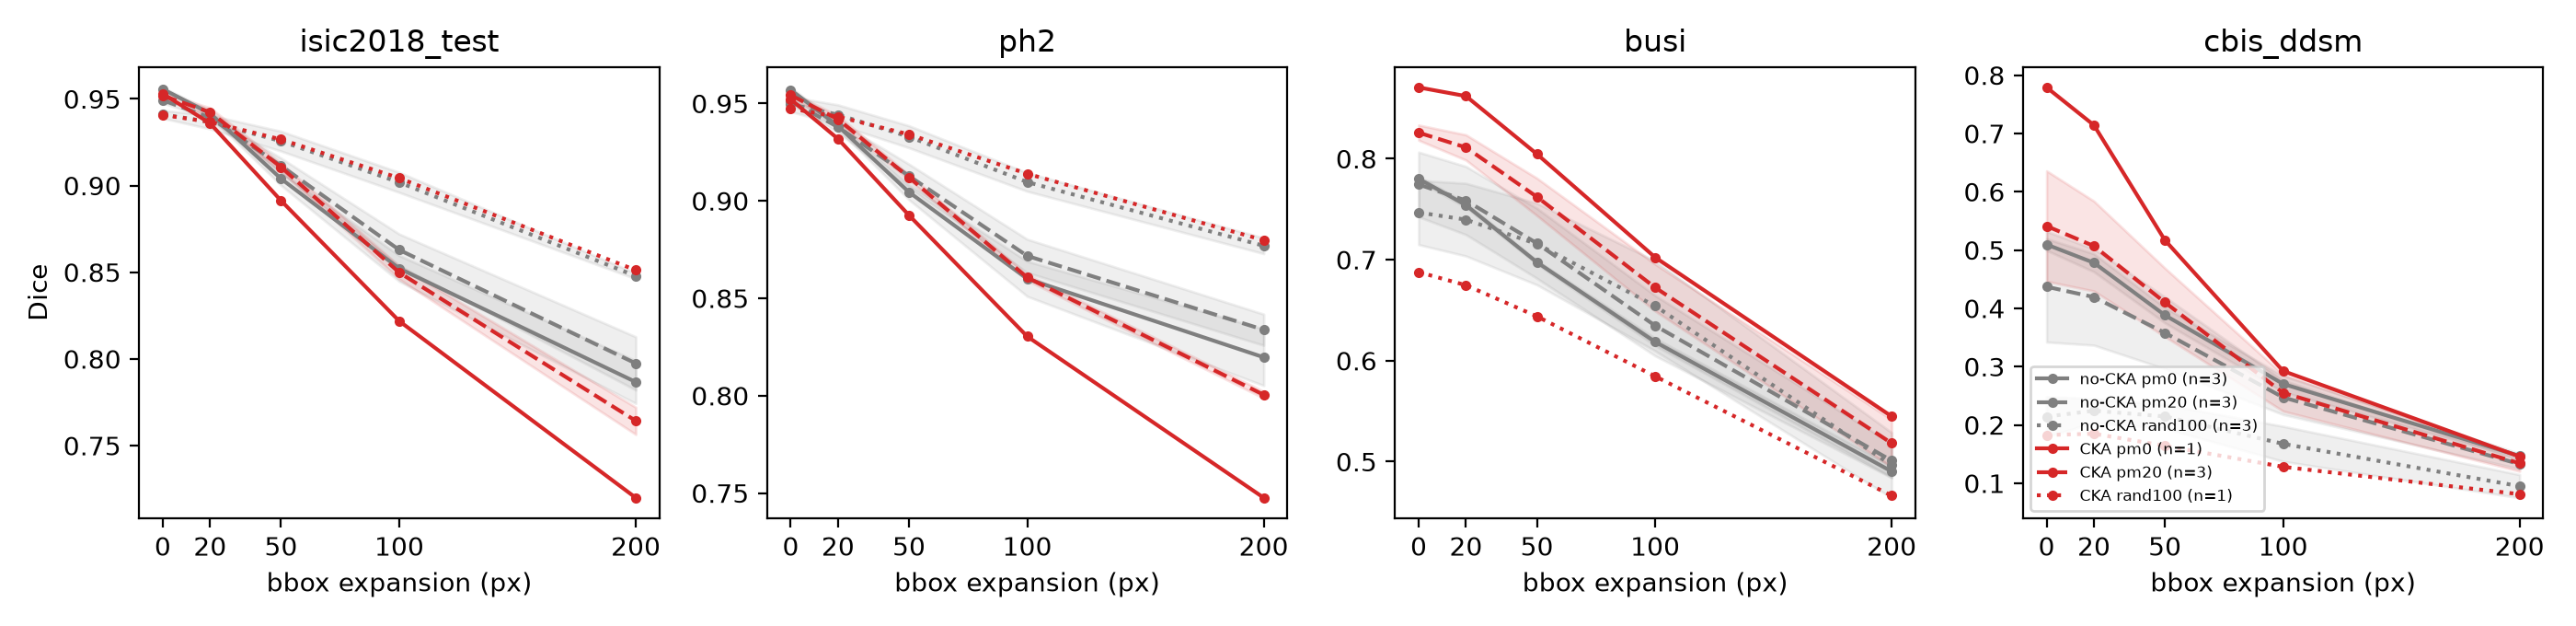
\includegraphics[width=\linewidth]{figures/robustness_six_curves.png}
  \caption{Dice against outward box expansion for LoRA with (red) and without (grey) the decoder CKA loss under three training regimes: tight (solid), 20\,px jitter (dashed), random jitter up to 100\,px (dotted). Bands: one std over three seeds where available.}
  \label{fig:curves}
\end{figure}

\emph{Prompt robustness:} In Fig.~\ref{fig:curves} the regularized pm20 model is the best of the six on both far-OOD sets at every expansion.The paired gain on BUSI falls from 0.053 at 20\,px to 0.017 at 200\,px, and on CBIS-DDSM from 0.088 to not significant. On the dermoscopy sets the sign flips beyond 50\,px (0.033 lower at 200\,px, $p < 10^{-20}$), so anchoring to a base trained with tight boxes inherits its sensitivity to loose boxes in-domain. The rand100 regime gains in-domain prompt robustness at a far-OOD price that the CKA loss makes worse.

\emph{Anchor placement ablations:} The hook ablation (LoRA, 20\,px training, tight-box , three seeds) separates the two halves of the model. With the loss on encoder activations alone, far-OOD Dice falls below the unregularized baseline, to $0.725 \pm 0.023$ on BUSI and $0.357 \pm 0.059$ on CBIS-DDSM (paired per-image loss 0.037 and 0.055, $p < 10^{-4}$), at unchanged IN-domain Dice. Decoder hooks give the gains of Table~\ref{tab:cka}. Anchoring both is best: $0.834 \pm 0.027$ and $0.626 \pm 0.098$, a paired gain over decoder hooks of 0.010 and 0.088 ($p < 10^{-4}$) and over no regularizer of 0.062 and 0.175, for a 0.003 in-domain cost. Seed spread on CBIS-DDSM is large for every arm (two trainings of one configuration reached 0.536 and 0.779), so we report paired statistics rather than best seeds. Overall, the decoder affects performance, and the encoder anchor helps only once the decoder is anchored.

\emph{Held-out far-OOD DMID mammography} is tested, which no model or probe has seen (269 images, tight boxes,), matching CBIS-DDSM: LoRA falls from a zero-shot 0.637 to 0.402, decoder-only, encoder-only and full fine-tuning reach 0.73, the decoder anchor lifts LoRA to 0.697 and encoder hooks alone give 0.366.

\begin{figure}[tbp]
  \centering
  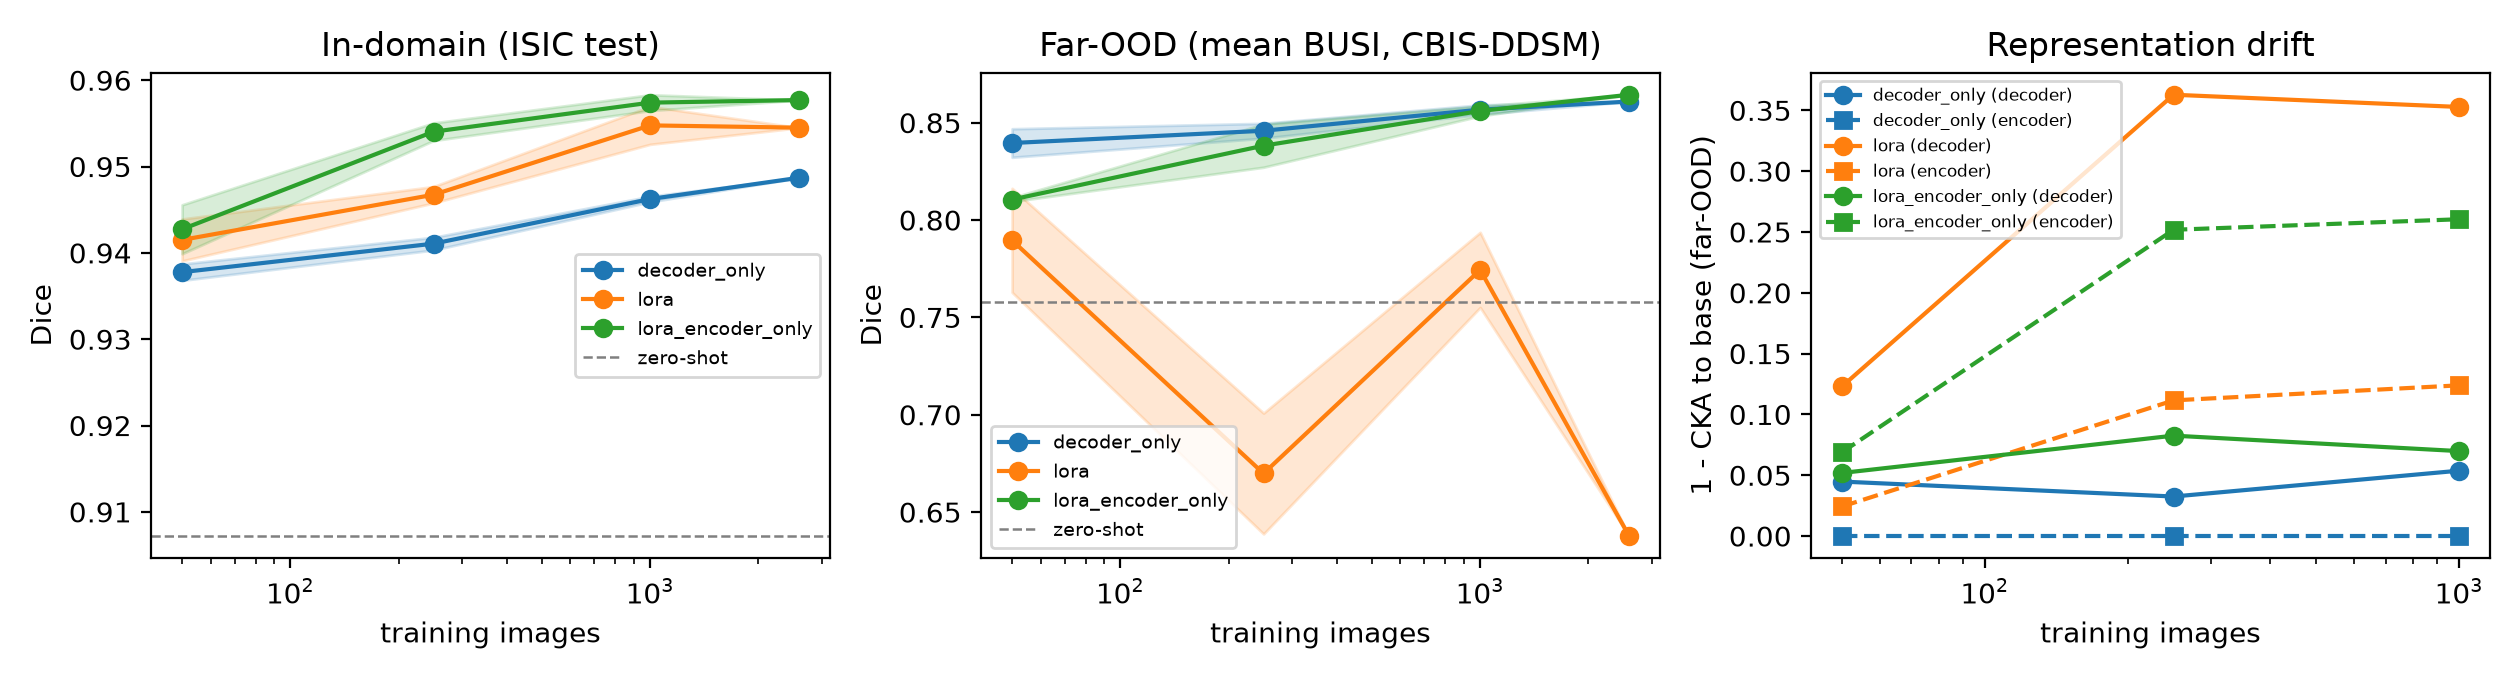
\includegraphics[width=\linewidth]{figures/budget_curves.png}
  \caption{Adapters trained for 6000 steps on nested subsets (log axis), zero-shot dashed. Left: in-domain Dice. Centre: far-OOD Dice (mean of BUSI, CBIS-DDSM). Right: far-OOD drift ($1 - \mathrm{CKA}$ to the base) of the decoder's upscaled embedding (circles) and encoder neck (squares, dashed). Dice: mean and std over three seeds at 50 to 1000 images; the 2595-image point and the drift panel are seed 0.}
  \label{fig:budget}
\end{figure}

\textbf{Adaptation Budget and Drift.} Figure~\ref{fig:budget} shows how the collapse depends on the budget and what changes inside the model. Decoder-only fine-tuning and encoder-only LoRA improve on both axes with every increase in budget and stay above the zero-shot far-OOD reference of 0.758 in every seed (0.840 to 0.861 and 0.811 to 0.864). LoRA with a trainable decoder is the only method that crosses it: already 0.02 to 0.05 below the others at 50 images ($0.790 \pm 0.027$, above zero-shot in each seed), it falls to $0.670 \pm 0.031$ at 250, below zero-shot in all three seeds, recovers to $0.774 \pm 0.019$ at 1000, above it in all three, and ends at 0.638 with all 2595 images, while its in-domain Dice rises monotonically. This is reflected in the drift panel on the right of Figure~\ref{fig:budget}. LoRA's far-OOD decoder drift triples between 50 and 250 images, from 0.12 to 0.36, exactly where its Dice collapses, and stays there. Decoder-only fine-tuning retrains every decoder weight yet keeps far-OOD decoder drift below 0.06 at all budgets, while encoder-only LoRA moves the encoder twice as much as LoRA (encoder drift 0.25 against 0.12) and keeps far-OOD decoder drift below 0.09. LoRA's far-OOD decoder drift triples between 50 and 250 images, from 0.12 to 0.36, coinciding with the sharp drop in far-OOD Dice. In contrast, decoder-only fine-tuning and encoder-only LoRA maintain low decoder drift and remain robust across budgets. Across these configurations, degradation emerges when the encoder and decoder are jointly adapted without an anchor. The dip at 250 images and partial recovery at 1000 are reproduced across all seeds, while the recovery occurs at essentially unchanged far-OOD decoder drift (0.35). Thus, decoder drift coincides with the onset of degradation but does not track its severity.

\begin{table}[tbp]
  \centering
  \caption{AUROC for detecting per-image failures (Dice $<$ 0.5) at tight boxes, mean $\pm$ std over three seeds (single value: seed 0 only): decoder drift (Eq.~\eqref{eq:drift}) versus the decoder's IoU estimate. Cells with fewer than 20 failures omitted; drift is zero by construction for zero-shot.}
  \label{tab:detect}
  \resizebox{\linewidth}{!}{\begin{tabular}{lcccccc}
\toprule
Method & \multicolumn{2}{c}{BUSI (far-OOD)} & \multicolumn{2}{c}{CBIS-DDSM (far-OOD)} & \multicolumn{2}{c}{DMID (held-out)} \\
 & drift & IoU head & drift & IoU head & drift & IoU head \\
\midrule
Zero-shot & -- & -- & -- & 0.49 & -- & 0.47 \\
Decoder-only FT & -- & -- & -- & -- & 0.39 $\pm$ 0.12 & 0.52 $\pm$ 0.09 \\
VPT-shallow & 0.95 $\pm$ 0.01 & 0.67 $\pm$ 0.02 & 0.72 $\pm$ 0.03 & 0.50 $\pm$ 0.06 & 0.57 $\pm$ 0.09 & 0.55 $\pm$ 0.12 \\
VPT-deep & 0.92 $\pm$ 0.01 & 0.64 $\pm$ 0.07 & 0.69 $\pm$ 0.03 & 0.50 $\pm$ 0.07 & 0.55 $\pm$ 0.09 & 0.50 $\pm$ 0.03 \\
LoRA & 0.96 $\pm$ 0.01 & 0.55 $\pm$ 0.16 & 0.80 $\pm$ 0.02 & 0.51 $\pm$ 0.09 & 0.69 $\pm$ 0.11 & 0.57 $\pm$ 0.16 \\
Encoder-only LoRA & -- & -- & -- & -- & 0.69 & 0.24 \\
Full FT & -- & -- & -- & -- & 0.57 $\pm$ 0.01 & 0.32 $\pm$ 0.03 \\
\bottomrule
\end{tabular}
}
\end{table}

\textbf{Label-Free Failure Signal.} The reliability of the per-image decoder drift as a label-free failure signal is investigated in a systematic manner.

\emph{Association of LoRA failures with decoder drift.} Over three seeds, LoRA fails on 61--82 of 647 BUSI images and 130--173 of 362 CBIS-DDSM images. Decoder drift ranks these failures with AUROC $0.96 \pm 0.01$ and $0.80 \pm 0.02$, respectively. On the held-out DMID dataset, 113--175 of 269 predictions fail, with decoder drift achieving AUROC $0.69 \pm 0.11$. The result does not hinge on the failure threshold (seed 0: AUROC 0.90 to 0.97 on BUSI and 0.73 to 0.82 on CBIS-DDSM for thresholds from 0.3 to 0.7). We translate the ranking quality into a review budget as follows (seed 0): Flagging the 20 percent of BUSI images with highest drift captures 87\,\% of LoRA's failures and leaves a failure rate of 1.5\,\% among the unflagged, from 9.4 percent overall. On CBIS-DDSM (42\,\% failures) flagging half captures 79\,\%. LoRA's IoU estimate is at chance on all three sets, collapsing after adaptation to a band between 0.4 and 0.6 regardless of mask quality ($0.55 \pm 0.16$, $0.51 \pm 0.09$, $0.57 \pm 0.16$).

\emph{Association of VPT failures with decoder drift.} VPT-shallow and VPT-deep failures are ranked by drift with AUROC $0.95 \pm 0.01$ and $0.92 \pm 0.01$ on BUSI and $0.72 \pm 0.03$ and $0.69 \pm 0.03$ on CBIS-DDSM, but on DMID only $0.57 \pm 0.09$ and $0.55 \pm 0.09$ (one seed of each at chance), although the per-image spread of drift is as wide as on CBIS-DDSM. Therefore, drift is not a universal signal: here, it is reliable for LoRA, weaker and seed-dependent on DMID, weak for VPT.

\emph{IoU estimate association to prompt, not modality:} Full fine-tuning and encoder-only LoRA produce only 2--14 failures on the far-OOD ladder datasets (tight-box prompts), too few for reliable failure-detection evaluation. Full fine-tuning's 50 to 52 DMID failures are missed by both signals in every seed (drift $0.57 \pm 0.01$, IoU $0.32 \pm 0.03$, below chance; encoder-only LoRA: 0.69 and 0.24). Under 50\,px jitter (seed 0), 220 to 236 CBIS-DDSM failures are detected by the IoU with AUROC 0.75 to 0.79, drift below chance (0.23 to 0.36). The IoU head flags a poor box, which every model can sense, rather than a modality it has never seen. Decoder drift identifies predictions for which the adapted decoder representations deviate substantially from those of the base model. However, its discriminative value diminishes when the decoder is either fully fine-tuned, causing representations to shift broadly across images, or constrained by CKA regularization to remain close to the base model (AUROC 0.35 and 0.46 on DMID, respectively). Neither signal constitutes an intrinsic self-assessment: computing drift requires an additional forward pass through the base model, and the reliability of both signals is evaluated retrospectively using ground-truth annotations.

\section{Conclusions and Future Work}
\label{sec:conclusion}

In this work, we investigated the role of representation drift in the far-OOD robustness of adapted MedSAM. Our results show that far-OOD degradation is closely associated with changes in the mask decoder when the encoder and decoder are jointly adapted. Preserving decoder representations through CKA regularization substantially improves far-OOD robustness, whereas constraining the encoder alone does not provide the same benefit. We further show that per-image decoder drift can serve as a useful label-free indicator of LoRA failures, although its effectiveness varies across adaptation strategies and domains. Future work should evaluate these findings across additional adaptation and target domains, as all models in this study were trained on dermoscopy. Further evaluation across seeds and distribution shifts is needed to establish the stability of the relationship between decoder drift and far-OOD performance. Future work should also reduce the computational overhead of CKA and drift-based failure detection, and develop representation-preserving objectives robust to prompt variation and adaptation strategy.

\bibliographystyle{splncs04}
\bibliography{refs}

\end{document}
